\section{Figures and their References}

\subsection{Example Figure}

Below is an example figure (Fig. \ref{fig:examplefig}) showing a diagram that might represent a process or a conceptual flow.

\begin{figure}[htbp]
    \centering
    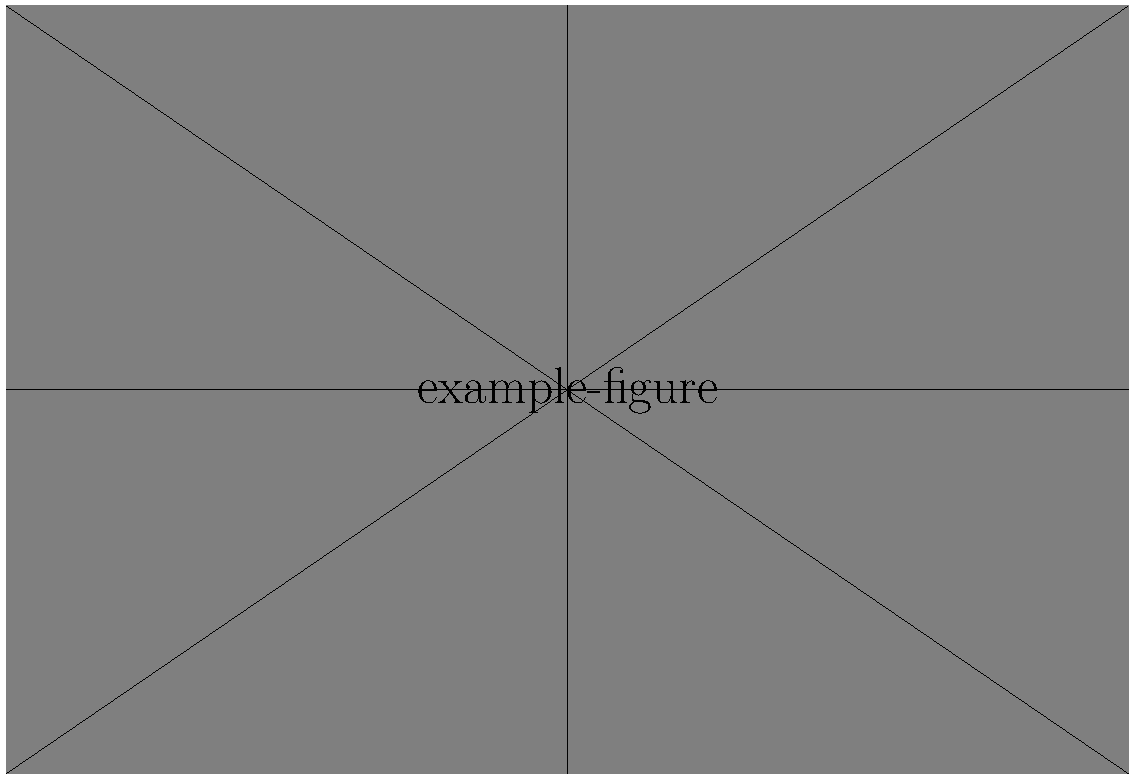
\includegraphics[width=0.8\linewidth]{example-figure}
    \caption{
        An example figure showing a conceptual diagram.
    }
    \label{fig:examplefig}
\end{figure}

\subsection{Subfigures}

Below is an example of subfigures (Fig. \ref{fig:examplesubfigures}), which contains 4 subfigures (Fig. \ref{fig:subfigure1}, Fig. \ref{fig:subfigure2}, Fig. \ref{fig:subfigure3}, and Fig. \ref{fig:subfigure4}).

\begin{figure}[htbp]
    \centering
    \subfloat[]{
        
\includegraphics[width=0.31\linewidth]{example-subfigure1}\label{fig:subfigure1}
    }
    \subfloat[]{
        
\includegraphics[width=0.23\linewidth]{example-subfigure2}\label{fig:subfigure2}
    }
    \subfloat[]{
        
\includegraphics[width=0.24\linewidth]{example-subfigure3}\label{fig:subfigure3}
    }
    \\
    \subfloat[]{
        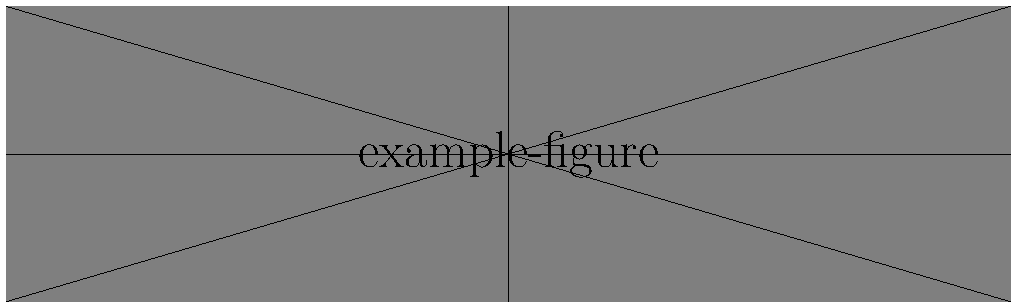
\includegraphics[width=0.8\linewidth]{example-subfigure4}\label{fig:subfigure4}
    }
    \caption{
        Example subfigures (a) Subfigure 1, (b) Subfigure 2, (c) Subfigure 3, and (d) Subfigure 4.
    }
    \label{fig:examplesubfigures}
\end{figure}